\chapter{Guida a Piatti Paralleli e Guida a Sezione Rettangolare}
\section{Caso TE}
Consideriamo, in un \textbf{mezzo omogeneo nel tempo} e nello \textbf{spazio}, \textbf{isotropo}, \textbf{spazialmente non dispersivo} e \textbf{senza perdite}, un'\textbf{onda piana incidente} su un piano \textbf{CEP}, con un angolo $\theta_i = \theta$ e \textbf{Incidenza TE}:
\begin{center}
    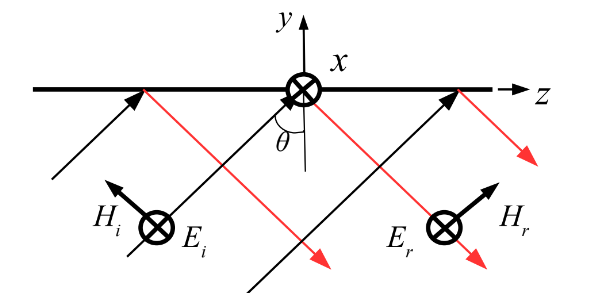
\includegraphics[width=.6\textwidth]{Images/figure42.png}
\end{center}
Il \textbf{campo elettrico} ha la sola componente \textbf{x}, \textbf{ortogonale} al piano (y,z):
\begin{equation*}
    \E^+_i = E^+_i \hat{i}_x = \hat{i}_x E^+_{i_0} e^{-j\k_i \cdot \r} = \hat{i}_x E^+_{i_0} e^{-j(k_y y + k_z z)}
\end{equation*}
Da notare che;
\begin{equation*}
    \begin{aligned}
    &\k_i = k_y \hat{i}_y + k_z \hat{i}_z\\
    &k_i^2 = k^2 = \w^2\epsilon \mu = k^2_y +k^2_z\\
    &k_y = k cos(\theta)\\
    &k_z = k sin(\theta)
    \end{aligned}
\end{equation*}
Per quanto riguarda l'\textbf{onda riflessa}:
\begin{equation*}
    \E^+_r = E^+_r \hat{i}_x = \hat{i}_x E^+_{r_0} e^{-j\k_r \cdot \r} = \hat{i}_x E^+_{r_0} e^{-j(-k_y y + k_z z)}
\end{equation*}
Dove:
\begin{equation*}
    \begin{aligned}
    &\k_r = - k_y \hat{i}_y + k_z \hat{i}_z\\
    &k_r^2 = k^2 = \w^2\epsilon \mu =  k^2_y +k^2_z\\
    &k_y = k cos(\theta)\\
    &k_z = k sin(\theta)
    \end{aligned}
\end{equation*}
Le \textbf{condizioni al contorno} del \textbf{CEP}, che si trova a coordinate (y=0) sono che la \textbf{componente tangente al piano del campo elettrico sia nulla}, ma nel caso in esame abbiamo che:
\begin{equation*}
    \E^+ (x,y,z) = \E_i^+ + \E_r^+ = \hat{i}_x (E^+_i + E_r^+)
\end{equation*}
è \textbf{tangente} al piano...\\ \\
Bisogna \textbf{imporre} che $\E_i^+ + \E^+_r = 0$ in y = 0:
\begin{equation*}
    \E^+ (x,0,z) = \hat{i}_x \left(E^+_{i_0} e^{-j k_z z} + E_{r_0}^+ e^{-j k_z z}\right) = 0
\end{equation*}
Che è \textbf{verificata} se e solo se $E_{r_0}^+ = - E^+_{i_0}$, quindi scriviamo in forma compatta:
\begin{squared}[violet]
\tag{X}
    \E^+ = E^+ \hat{i}_x = - 2j E^+_{i_0} sin(k_y y) e^{-j k_z z} \hat{i}_x
\end{squared}
 Quindi $\E^+$ si \textbf{annulla} per y = 0, ma anche \textbf{ogni}:
 \begin{equation*}
     y = y_n : \quad k_y y_n = n\pi
 \end{equation*}
 Questa espressione ci dice che se poniamo \textbf{un altro CEP} ad una distanza $a = y_n$ dal piano y=0, questo piano \textbf{non perturba} il campo $(X)$, o in altri termini se cerchiamo le \textbf{soluzioni delle equazioni di Maxwell in assenza di sorgenti}, tra due \textbf{CEP} distanti a (e supponiamo campo TE) ottengo l'espressione $(X)$ che tra i due piani \textbf{rispetta le equazioni di Maxwell in assenza di sorgenti}.\\ \\
 Fissando ora a:
 \begin{equation*}
     k_y a = n\pi \implies k_y = k_n = n \frac{\pi}{a}
 \end{equation*}
Cioè per angoli:
\begin{equation*}
    \theta = \theta^{(n)} = acos\left(\frac{k_n}{k}\right) = acos\left(\frac{n\pi}{a k}\right) = n \frac{\lambda}{2a}
\end{equation*}
Calcoliamo ora il \textbf{campo magnetico} partendo da \textbf{Faraday-Lenz}:
\begin{equation*}
    \rot{\E} = - j\w \mu \H \implies \left(\nabla_t - jk_z \hat{i}_z\right) \times \E_t = -j \w \mu \H_t - j \w \mu H_z \hat{i}_z
\end{equation*}
Da cui:
\begin{equation*}
    \begin{dcases}
    k_z \hat{i}_z \times \E_t = \w \mu \H_t\\
    \nabla_t \times \E_t = - j\w \mu H_z \hat{i}_z
    \end{dcases}
\end{equation*}
La prima ci mostra che $\H_t$ è \textbf{proporzionale} ad $\E_t$ \textbf{ruotato} di $\pi/2$.\\ \\
Ora sostituiamo $(X)$:
\begin{equation*}
    k_z \underbrace{\hat{i}_z \times \hat{i}_x}_{\hat{i}_y} E^+ = k_z \hat{i}_y E^+ = - 2 j k_z E^+_{i_0} sin(k_y y) e^{-j k_z z} \hat{i}_y = \w \mu \H_t
\end{equation*}
Quindi:
\begin{equation*}
    \H_t = H_y \hat{i}_y = -2j\frac{k_z}{\w \mu} E^+_{i_0} sin(k_y y) e^{-j k_z z}\hat{i}_y
\end{equation*}
Dalla seconda invece, calcoliamo la \textbf{componente longitudinale} di $\H$:
\begin{equation*}
    - j\w \mu H_z \hat{i}_z =  \nabla_t \times \E_t
\end{equation*}
\begin{equation*}
    - j\w \mu H_z = \hat{i}_z \cdot \nabla_t \times \E_t = \nabla_t \cdot (\E_t \times \hat{i}_z)
\end{equation*}
Sostituiamo $(X)$:
\begin{equation*}
\begin{aligned}
    &\nabla_t \cdot \left(2jE^+_{i_0} sin(k_y y) e^{-j k_z z}\hat{i}_y\right) =\\
    &= \frac{\partial}{\partial y} \left(2j E^+_{i_0} sin(k_y y) e^{-j k_z z}\right) = \\
    &= 2j k_y E^+_{i_0} cos(k_y y) e^{-j k_z z} =  - j\w \mu H_z
\end{aligned}
\end{equation*}
Quindi:
\begin{equation*}
    H_z = -2 \frac{k_y}{\w \mu} E^+_{i_0}cos(k_y y) e^{-j k_z z}
\end{equation*}
Quindi \textbf{tra due CEP paralleli}, in \textbf{assenza di sorgenti}, si può \textbf{propagare un campo elettromagnetico}.\\ \\
Definiamo:
\begin{equation*}
\begin{dcases}
    A^+_E = -2j E^+_{i_0}\\
    A^+_H = -2j\frac{k_z}{\w \mu} E^+_{i_0} =  -2j\frac{k_z}{\w \mu} \zeta H^+_{i_0} =  -2j\frac{k_z}{k} H^+_{i_0}
\end{dcases}
\end{equation*}
Dato che:
\begin{equation*}
    \begin{dcases}
    k = \w \sqrt{\epsilon \mu}\\
    \zeta = \frac{\mu}{\sqrt{\epsilon \mu}}
    \end{dcases}
\end{equation*}
Quindi possiamo scrivere il \textbf{campo elettrico} \textbf{tra i due CEP} come:
\begin{equation*}
\begin{dcases}
    \E^+ = A^+_E sin(k_y y) e^{-j k_z z} \hat{i}_x\\
    \H^+_t = \frac{k_z}{\w \mu} \hat{i}_z \times \E^+_t = \frac{k_z}{\w \mu} A^+_E e^{-j k_z z}sin(k_y y) \hat{i}_y = A^+_H e^{-j k_z z}sin(k_y y) \hat{i}_y\\
    H^+_z = -j \frac{k_y}{\w \mu} A^+_E cos(k_y y) e^{-j k_z z} = -j \frac{k_y}{k_z} A^+_H cos(k_y y) e^{-j k_z z}
\end{dcases}
\end{equation*}
Dove:
\begin{equation*}
    k_y = k_n = n \frac{\pi}{a}, \quad k_z = \sqrt{k^2 - k_n^2} = \sqrt{k^2 -  \left(n \frac{\pi}{a}\right)^2}
\end{equation*}
Diciamo però che questo campo \textbf{è possibile solo per alcuni valori} di $k_y$ e $k_z$, dove:
\begin{itemize}
    \item $k_y$ \textbf{autovalore trasverso}
    \item $k_z$ \textbf{autovalore longitudinale}
\end{itemize}
Questo campo è \textbf{confinato nei due CEP} e si propaga verso Z, longitudinalmente al piano (x,y), \textbf{ma questo piano è infinito!!}\\ \\
Quindi \textbf{non è realizzabile}...\\ \\
Infatti se calcoliamo il \textbf{flusso di potenza} per una generica z \textbf{otterremo un flusso di potenza infinito!} Anche se la \textbf{densità di potenza} è \textbf{finita}...\\ \\
Osservando le \textbf{equazioni dei campi} che abbiamo ricavato notiamo che il \textbf{campo elettrico} è tutto nella direzione x.\\
Quindi possiamo mettere \textbf{altri due CEP paralleli all'asse y}, separati da una distanza \textbf{b} in modo tale da \textbf{non perturbare le equazioni ottenute}:
\begin{center}
    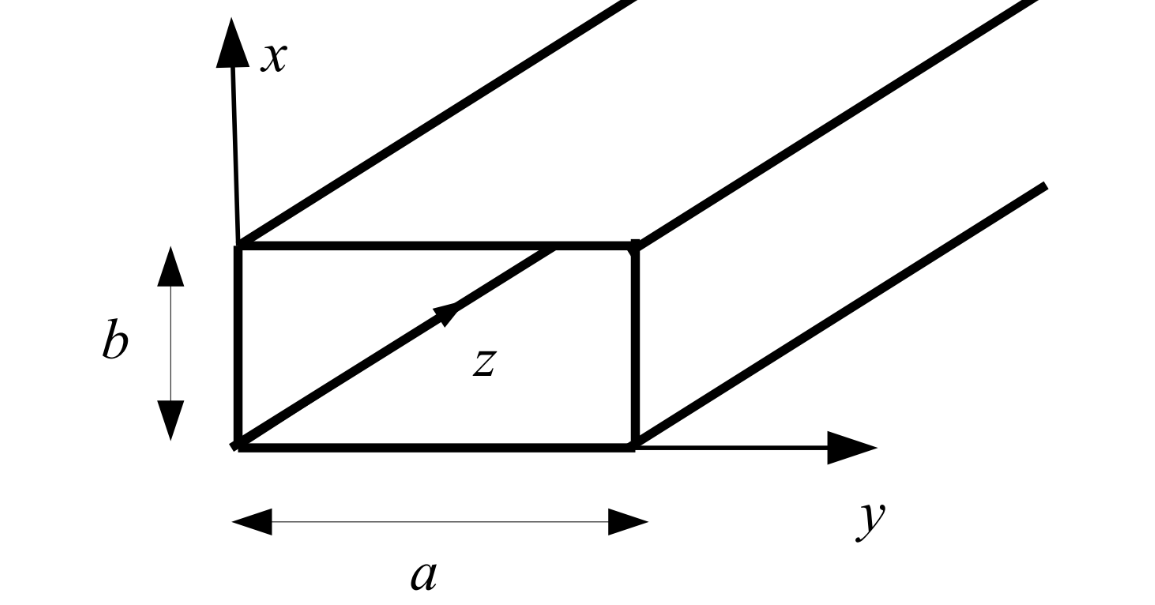
\includegraphics[width=.6\textwidth]{Images/figure44.png}
\end{center}
Possiamo anche considerare il \textbf{campo nullo all'esterno di questo "tubo"}.\\
Mentre il \textbf{campo all'interno rispetta le condizioni a contorno}, ovvero \textbf{componenti tangenti del campo elettrico nulle sui conduttori}.\\ \\
Se ora calcolassimo il \textbf{flusso di potenza} attraverso una qualsiasi sezione trasversa, sarebbe \textbf{finito}.\\ \\
Questa \textbf{guida metallica NON TEM} prende il nome di \textbf{guida metallica rettangolare}.\\ \\
Possiamo scomporre il \textbf{campo elettrico} nella guida come:
\begin{equation*}
    \begin{dcases}
        \E^+_i = E^+_{ix} \hat{i}_x = E^+_{i0} e^{-j(k_y y + k_z z)} \hat{i}_x \\
        \E^+_r = E^+_{rx} \hat{i}_x = E^+_{r0} e^{-j(-k_y y + k_z z)} \hat{i}_x
    \end{dcases}
\end{equation*}
Possiamo però considerare anche:
\begin{equation*}
    \begin{dcases}
        \E^-_i = E^-_{ix} \hat{i}_x = E^-_{i0} e^{j(-k_y y + k_z z)} \hat{i}_x \\
        \E^-_r = E^-_{rx} \hat{i}_x = E^-_{r0} e^{j(k_y y + k_z z)} \hat{i}_x
    \end{dcases}
\end{equation*}
Sia quelle sopra che queste sotto, sommandosi \textbf{verificano le condizioni a contorno sui CEP}:
\begin{equation*}
    \E^- = \E^-_i + \E^-_r = \E^- \hat{i}_x  = -2jE^-_{i0} sin(k_y y) e^{jk_z z} \hat{i}_x = A^-_E sin(k_y y) e^{jk_z z} \hat{i}_x 
\end{equation*}
Discorso analogo per $\H^-$, ma si può notare che basta cambiare di segno $k_z$:
\begin{equation*}
    \begin{dcases}
    \H^-_t = A^-_H sin(k_y y) e^{jk_z z} \hat{i}_y\\
    H_z^- = j \frac{k_y}{k_z} A^-_H cos(k_y y) e^{jk_z z}
\end{dcases}
\end{equation*}
Riassumendo, nella \textbf{guida}, in \textbf{assenza di sorgenti}, per ogni $k_n$ troviamo un \textbf{campo TE} ($E_0$):
\begin{equation*}
\begin{dcases}
    \E^+ = \left(A^+_E e^{-j k_z z} +  A^-_E e^{j k_z z} \right)   sin(k_y y) \hat{i}_x\\
    \H^+_t = \left(A^+_E e^{-j k_z z} +  A^-_E e^{j k_z z} \right) \frac{k_z}{\w \mu} sin(k_y y) \hat{i}_y\\
    H^+_z = -j \frac{k_y}{\w \mu} \left(A^+_E e^{-j k_z z} +  A^-_E e^{j k_z z} \right) cos(k_y y) 
\end{dcases}
\end{equation*}
Possiamo ora notare che $\E_t$ e $\H_t$ sono costituite dal prodotto di una \textbf{ampiezza scalare dipendente da z}, per una \textbf{funzione vettoriale che dipende solo da y in questo caso}, ma come vedremo può dipendere anche da x e y:
\begin{equation*}
    \begin{dcases}
        \E = \left(V^+ e^{-j k_z z} +  V^- e^{j k_z z} \right) \e(x,y) = V(z) \e(x,y)\\
        \H_t = \left(I^+ e^{-j k_z z} + I^-  e^{j k_z z} \right) \h_t(x,y) = I(z) \h_t(x,y)
    \end{dcases}
\end{equation*}
Questa \textbf{fattorizzazione} \textbf{non è univoca}, possiamo infatti moltiplicare $V(z)$ (o $I(z)$) e dividere $\e_t$ (o $\h_t$) per una stessa \textbf{costante} chiamate \textbf{costanti di separazione}, ed ottenere lo stesso campo.\\ \\
Una di queste costanti può essere scelta imponendo:
\begin{equation*}
    \e_t = \h_t \times \hat{i}_z
\end{equation*}
Quindi:
\begin{equation*}
    \begin{dcases}
        V^+ = I^+ Z_{TE}\\
        V^- =- I^- Z_{TE}\\
        Z_{TE} = \frac{V^+}{I^+} = \frac{A^+_E}{A^+_E \cdot \frac{k_z}{\w \mu}} = \frac{\w \mu}{k_z}
    \end{dcases}
\end{equation*}
Notiamo in particolar modo che l'\textbf{ampiezza del campo elettrico trasverso} ($V(z)$) e del \textbf{campo magnetico trasverso} ($I(z)$) variano lungo la guida allo stesso modo della \textbf{tensione} e della \textbf{corrente} lungo una \textbf{linea di trasmissione}:
\begin{equation*}
    \begin{dcases}
        V(z) =V^+ e^{-jk_z z} + V^- e^{jk_z z}\\
        I(z) =\frac{V^+}{Z_{TE}} e^{-jk_z z} - \frac{V^-}{Z_{TE}} e^{jk_z z}
    \end{dcases}
\end{equation*}
Con: $Z_{TE} =  \frac{k_z}{\w \mu}, \quad k_z = \sqrt{k^2 - \left(n - \frac{\pi}{a}\right)^2}$\\ \\
Queste \textbf{ampiezze} rispettano le \textbf{equazioni delle linee}:
\begin{equation*}
    \begin{dcases}
        \frac{dV}{dZ} = -j \w \mu I = -j \w L_{eq} I\\
        \frac{dI}{dZ} = -j \w \frac{k_z^2}{\w^2 \mu} V = -j \w C_{eq} V
    \end{dcases}
\end{equation*}
Possiamo quindi \textbf{associare} alla \textbf{propagazione in guida d'onda metallica}, per un fissato $k_n$, \textbf{la linea  TEM sopra descritta}.\\ 
Da ricordare però che in questo caso \textbf{V non è una vera tensione} e \textbf{I non è una vera corrente}.\\ \\
Possiamo però creare un'altra analogia fissando la \textbf{seconda costante di separazione}, imponendo:
\begin{equation*}
    \int_S \e_t \times \h_t \cdot \hat{i}_z dS = 1
\end{equation*}
Dove S è la sezione trasversa della guida.\\ \\
La \textbf{potenza} in una generica sezione z sarà:
\begin{equation*}
    \begin{aligned}
        P(z) &= \int_S \frac{1}{2} \E \times \H^* \cdot \hat{i}_z dS =  \int_S \frac{1}{2} \E_t \times \H_t^* \cdot \hat{i}_z dS =\\
        &= \int_S  V(z) \h_t \times I^*(z) \h_t \cdot \hat{i}_z dS = \frac{1}{2} V(z) I^*(z)
    \end{aligned}
\end{equation*}
Notiamo che la \textbf{normalizzazione} può anche essere riscritta come:
\begin{equation*}
    \int_S \e_t \times \h_t \cdot \hat{i}_z dS= \int_S \underbrace{\h_t \times  \hat{i}_z}_{\e_t} \cdot \e_t dS = \int_S \e_t  \cdot \e_t dS = 1
\end{equation*}
Analogamente:
\begin{equation*}
    \int_S \h_t  \cdot \h_t dS = 1
\end{equation*}
Quindi possiamo ricavare:
\begin{equation*}
    \begin{dcases}
        \e_t = \sqrt{\frac{2}{ab}} sin\left(n \frac{\pi}{a} y\right) \hat{i}_x\\
        \h_t = \sqrt{\frac{2}{ab}} sin\left(n \frac{\pi}{a} y\right) \hat{i}_y\\
        h_z = -j \frac{k_y}{k_z} \sqrt{\frac{2}{ab}} cos\left(n \frac{\pi}{a} y\right)
    \end{dcases}
\end{equation*}
Infine notiamo una \textbf{relazione} tra questi campi:
\begin{equation*}
    \nabla_t h_z = j \frac{k_y}{k_z} k_y \underbrace{\sqrt{\frac{2}{ab}}  sin\left(k_y y\right) \hat{i}_y}_{\h_t} = j \frac{k^2_y}{k_z}\h_t = j  \frac{k^2_y}{k_z} \hat{i}_z \times \e_t
\end{equation*}
Ragionando possiamo dire che è possibile fare dei calcoli del tutto analoghi ruotando la guida e considerando un'onda che incide sul piano (y,z), anzichè sul piano (x,z).\\ 
Facendo le stesse \textbf{considerazioni} e \textbf{normalizzazioni} avremo:
\begin{equation*}
    \nabla_t h_z = - j \sqrt{\frac{2}{ab}} \frac{k_x}{k_z} \left(m \frac{\pi}{b}\right) sin\left(m \frac{\pi}{b}\right)\hat{i}_x = j  \frac{k^2_x}{k_z} \h_t = j \frac{k^2_x}{k_z} \hat{i}_z \times \e_t
\end{equation*}
Questa espressione, come quella del primo caso, ci dice che le \textbf{componenti dei campi trasversi} possono essere ricavati mediante le \textbf{componenti longitudinali} a patto che esse \textbf{rispettino le condizioni al contorno} che per $h_z$ sarebbero \textbf{derivata nulla sui conduttori}.\\ \\
Assumiamo per $h_z$ una forma generale:
\begin{equation*}
    h_z = j acos\left(n \frac{\pi}{a} y\right) cos\left(m \frac{\pi}{b} x\right)
\end{equation*}E valutiamone il gradiente:
\begin{equation*}
\begin{aligned}
    \nabla_t h_z &= -j A \left[\left(n \frac{\pi}{a}\right) sin \left(n \frac{\pi}{a} y\right) cos\left(m \frac{\pi}{b} x\right)\hat{i}_y + \right. \\
    &\left. + \left(m \frac{\pi}{b} \right) cos\left(n \frac{\pi}{a} y\right) sin\left(m \frac{\pi}{b} x\right) \hat{i}_x\right]
\end{aligned}
\end{equation*}
Confrontandola con le altre possiamo asserire che $\hat{i}_z \times \nabla_t h_z$ \textbf{soddisfa le condizioni a contorno}:\footnote{A e B sono costanti di normalizzazione}
\begin{equation*}
    \e_t = j C \hat{i}_z \times \nabla_t h_z = B \left[sin \left(n \frac{\pi}{a} y\right) cos\left(m \frac{\pi}{b} x\right)\hat{i}_x
    - cos\left(n \frac{\pi}{a} y\right) sin\left(m \frac{\pi}{b} x\right) \hat{i}_y\right]
\end{equation*}
Perchè così le \textbf{componenti tangenti del campo elettrico} si \textbf{annullano sulle pareti} del conduttore!! Infatti:
\begin{equation*}
    \begin{dcases}
        e_x(x,0) = e_x(x,a) = 0\\
        e_y(0,y) = e_y(b,y) = 0
    \end{dcases}
\end{equation*}
Ce ne sono due perchè l'onda incide su tutti e 4 i piani, quindi vuol dire che $\k$ avrà 3 componenti:
\begin{equation*}
    \k = k_x \hat{i}_x + k_y  \hat{i}_y + k_z \hat{i}_z = \k_{t_{nm}} + k_z \hat{i}_z
\end{equation*}
Dove:
\begin{equation*}
    \begin{dcases}
        k_x = m \frac{\pi}{b}\\
        k_y = n \frac{\pi}{a}\\
        k_{z_{nm}} = \sqrt{k^2 - k^2_{t_{nm}}} = \sqrt{k^2 - \left(m \frac{\pi}{b}\right)^2 - \left(n \frac{\pi}{a}\right)^2}
    \end{dcases}
\end{equation*}
Quindi in una \textbf{guida metallica rettangolare} si possono propagare una \textbf{doppia infinità numerabile di modi} \textbf{ad ogn'uno dei quali possiamo associare una linea di trasmissione equivalente} con i seguenti parametri:
\begin{equation*}
    L_{eq} = \mu, \quad C_{eq}= \frac{k^2_{z_{nm}}}{\w^2 \mu}
\end{equation*}
\textbf{In particolare il modo che si propaga con il $k_z$ più grande è detto modo fondamentale.}
\subsection{Il Fenomeno del Cut-Off nelle Guide Metalliche}
Consideriamo il seguente \textbf{modo (n,m)} costituito dalle seguenti \textbf{onde di tensione} e di \textbf{corrente} equivalenti che si propagano in una \textbf{guida a sezione rettangolare} con \textbf{costante di propagazione} $K_{z_{n,m}}$ (consideriamo per semplicità solo quelle nella direzione positiva di z):
\begin{equation*}
\begin{dcases}
    V(z) = V^+ e^{-jK_{z_{n,m}}z}\\
    I(z) = \frac{V^+}{Z_{TE}^{n,m}} e^{-jK_{z_{n,m}}z}
\end{dcases}
\end{equation*}
Dove:
\begin{equation*}
    K_{z_{n,m}} = \sqrt{K^2 - K_{t_{n,m}}^2}
\end{equation*}
In particolare:
\begin{equation*}
    K^2 = \omega^2 \epsilon \mu 
\end{equation*}
Che è \textbf{funzione} di $\omega$, mentre $K^2_{t_{n,m}}$ è \textbf{indipendente} da $\omega$, quindi possiamo calcolare la particolare \textbf{pulsazione} $\omega_{t_{n,m}}$ che \textbf{annulla} $K_{z_{n,m}}$:
\begin{equation*}
    \omega_{t_{n,m}} = \frac{K_{t_{n,m}}}{\epsilon \mu}
\end{equation*}
Per \textbf{pulsazioni maggiori} di $\omega_{t_{n,m}}$ il radicando è \textbf{positivo} e quindi la radice ammette una \textbf{determinazione reale positiva}.\\ 
Tuttavia per \textbf{pulsazioni minori} di $\omega_{t_{n,m}}$ il radicando è \textbf{negativo} e quindi la radice ammette \textbf{due determinazioni immaginarie}, dove:
\begin{itemize}
    \item La determinazione \textbf{immaginaria} \textbf{positiva} corrisponde ad un \textbf{campo che cresce nella direzione positiva delle z}, ma il mezzo è \textbf{passivo} quindi \textbf{non è una soluzione fisica};
    \item La determinazione \textbf{immaginaria} \textbf{negativa} corrisponde ad un \textbf{campo che si attenua lungo le z positive}, ma questa attenuazione è di tipo \textbf{reattivo}.
\end{itemize}
Possiamo quindi dire che:
\begin{equation*}
\begin{dcases}
    K_{z_{n,m}} = \sqrt{K^2 - K_{z_{n,m}}^2} = \beta_{n,m},\; sse \ \omega > \omega_{t_{n,m}}\\
    K_{z_{n,m}} = \sqrt{K^2 - K_{z_{n,m}}^2} = -j \alpha_{n,m},\; sse \ \omega < \omega_{t_{n,m}}
\end{dcases}
\end{equation*}
Quindi \textbf{ogni modo si propaga solo per pulsazioni superiori alla pulsazione} $\omega_{t_{n,m}}$ detta \textbf{pulsazione di taglio del modo}.\\ \\
Il modo che la \textbf{pulsazione di taglio} \textbf{più bassa} (che quindi si propaga prima) è il \textbf{modo fondamentale}.\\ \\

Per esempio, considerando una \textbf{guida rettangolare metallica} con $a > b$, il \textbf{modo fondamentale} è il $TE_{10}$:
\begin{equation*}
    K_{t_{10}} = \frac{\pi}{a}
\end{equation*}
\begin{equation*}
    \omega_{t_{10}} = \frac{\pi}{a \epsilon \mu}
\end{equation*}
\begin{equation*}
    K_{z_{10}} = \sqrt{K^ - \left(\frac{\pi}{a}\right)^2}
\end{equation*}

Una cosa interessante che possiamo elaborare da queste informazioni è che una \textbf{guida metallica} \textbf{semplicemente} \textbf{connessa} si comporta come un \textbf{filtro passa alto} dato che al di sotto della \textbf{pulsazione di taglio} non lascia propagare nulla.\\ \\

Valutiamo ora il \textbf{flusso di potenza} ad una qualsiasi sezione della \textbf{guida}:
\begin{equation*}
\begin{aligned}
    P(z) &= \int_S \frac{1}{2} \E \times \H^* \cdot \hat{i}_z dS = \int_S \frac{1}{2} \E_t \times \H_t^* \cdot \hat{i}_z dS = \\
    &= \int_S V(z) \e_t \times I^*(z) \h_t \cdot \hat{i}_z = \frac{1}{2} V(z) I^*(z)
\end{aligned}
\end{equation*}
dove per $\omega > \omega_{t_{n,m}} \implies K_{z_{n,m}} = \beta_{n,m}$:
\begin{equation*}
    P = \frac{1}{2} V^+ e^{-j K_{z_{n,m}}z}  \ \frac{V^{+^*}}{Z_{TE}^{{n,m}^*}} e^{j K^*_{z_{n,m}}z} = \frac{1}{2}|V^+|^2 \frac{\beta_{n,m}}{\omega \mu} \footnote{dove $Z_{TE} = \frac{\omega \mu}{K_z}$}
\end{equation*}
Quindi in questo caso abbiamo una \textbf{potenza attiva}, mentre nel caso contrario $\omega < \omega_{t_{n,m}} \implies K_{z_{n,m}} = - j \alpha_{n,m}$:
\begin{equation*}
    P = \frac{1}{2} V^+ e^{-j K_{z_{n,m}}z}  \ \frac{V^{+^*}}{Z_{TE}^{{n,m}^*}} e^{j K^*_{z_{n,m}}z} = \frac{1}{2} j\frac{\alpha_{n,m}}{\omega \mu} |V^+|^2  e^{-2\alpha_{n,m}z}
\end{equation*}
Quindi in questo caso abbiamo una \textbf{potenza alla generica sezione puramente reattiva} e diminuisce con z.

\section{Caso TM} 
\begin{center}
   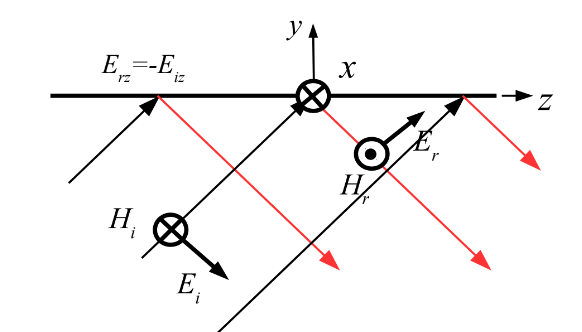
\includegraphics[width=.8\textwidth]{Images/figure46.png}
\end{center}
\begin{equation*}
    \begin{dcases}
    \E_i = E_{i_0} e^{-j(k_y y - k_z z)}\\
    E_{i_z} = E_{i_{0_z}} e^{-(jk_y y - k_z z)}\\
    \E_z = E_{i_{0_z}} e^{-j k_z z} \left(e^{-j k_y y} - e^{jk_y y}\right) = - E_{i_{0_z}} e^{-j k_z z}  2 j sin(k_y y)
    \end{dcases}
\end{equation*}
Mentre il campo elettrico riflesso sarà:
\begin{equation*}
\begin{dcases}
    \E_r = E_{r_0} e^{j(k_y y - k_z z)}\\
    E_{r_z} = \underbrace{E_{r_{0_z}}}_{-E_{i_{0_z}}} e^{j(k_y y - k_z z)}
\end{dcases}
\end{equation*}
Possiamo fare questa sostituzione perchè sul contorno la somma:
\begin{equation*}
    E_{i_z} + E_{r_z} = 0
\end{equation*}
Quindi se $k_y = \frac{n\pi}{a}$ posso mettere un altro piano rispettando le condizioni.

